\documentclass{article} % For LaTeX2e
\usepackage{nips13submit_e,times}
\usepackage{hyperref}
\usepackage{graphicx}
\usepackage{url}
\usepackage{placeins}
%\documentstyle[nips13submit_09,times,art10]{article} % For LaTeX 2.09


\title{CS 229 Milestone}

\author{Matthew Staib, Lennart Jansson, and Edward Dai}

% The \author macro works with any number of authors. There are two commands
% used to separate the names and addresses of multiple authors: \And and \AND.
%
% Using \And between authors leaves it to \LaTeX{} to determine where to break
% the lines. Using \AND forces a linebreak at that point. So, if \LaTeX{}
% puts 3 of 4 authors names on the first line, and the last on the second
% line, try using \AND instead of \And before the third author name.

\newcommand{\fix}{\marginpar{FIX}}
\newcommand{\new}{\marginpar{NEW}}

\nipsfinalcopy % Uncomment for camera-ready version

\begin{document}

\maketitle

\section{A short note about our topic}
Originally, we were planning to classify popular music by country of origin
using audio features. For example, we intended to cluster based on these
features and hoped to observe clusters corresponding to geographic origin.
However, after some reconsidering, we decided that this was infeasible since we
expected similarity between songs to be more closely tied to genre and other
factors instead of country of origin. We also had problems finding a large
dataset where we would have been able to choose the audio features ourselves
(e.g. The Million Song Dataset is quite vast and has audio features, but not the
original audio).

We still wanted to work on a project related to music and music analysis, but
decided that it would be more feasible to consider a problem with a cleaner
dataset. One of our group members had previously experimented with a dataset of
folk dance music where melodies are stored in a commonly used score notation
(ABC notation).

\section{Introduction}
Most folk dance music contains two musical themes; the tune begins with one
musical theme, progresses to another, and then repeats the first. The first
section is typically called the $A$ section while the second is called the $B$
section. Our goal is to understand, at a quantitative level, the relationship
between $A$ sections and $B$ sections. In the long term, for example, we want to
be able to, given an $A$ section, automatically generate a musically appropriate
$B$ section.

In working towards this goal, we need to understand both the relationship
between the $A$ and $B$ section of a given folk song as well as the differences
between $A$ and $B$ sections of such music in general. 

\section{Dataset}

%TODO: Maybe do something with citing?
We are using the tunes dataset from The Session (\texttt{thesession.org}). The
Session is an online community of people who are interested in playing Irish
folk music and cataloguing traditional Irish tunes for others to learn. These
tunes include various dance forms, such as jigs, reels, waltzes, and slides.
Available on their website is a set of roughly 21 thousand dance tune settings
in ABC notation, a human-readable symbolic music data format in plain text. The
ABC files are easily parsed and manipulated symbolically for feature extraction.
\FloatBarrier
\begin{figure}
  \begin{verbatim}
X: 1
T: Drowsy Maggie
R: reel
M: 4/4
L: 1/8
K:Edor
|:E2BE dEBE|E2BE AFDF|E2BE dEBE|BABc dAFD:|
K:D
d2fd c2ec|defg afge|d2fd c2ec|BABc dAFA|
d2fd c2ec|defg afge|afge fdec|BABc dAFD|
  \end{verbatim}
  \caption{\textit{Drowsy Maggie}, an example of a tune in ABC notation from
  \texttt{thesession.org}.}
\end{figure}
\begin{figure}
  \begin{center}
    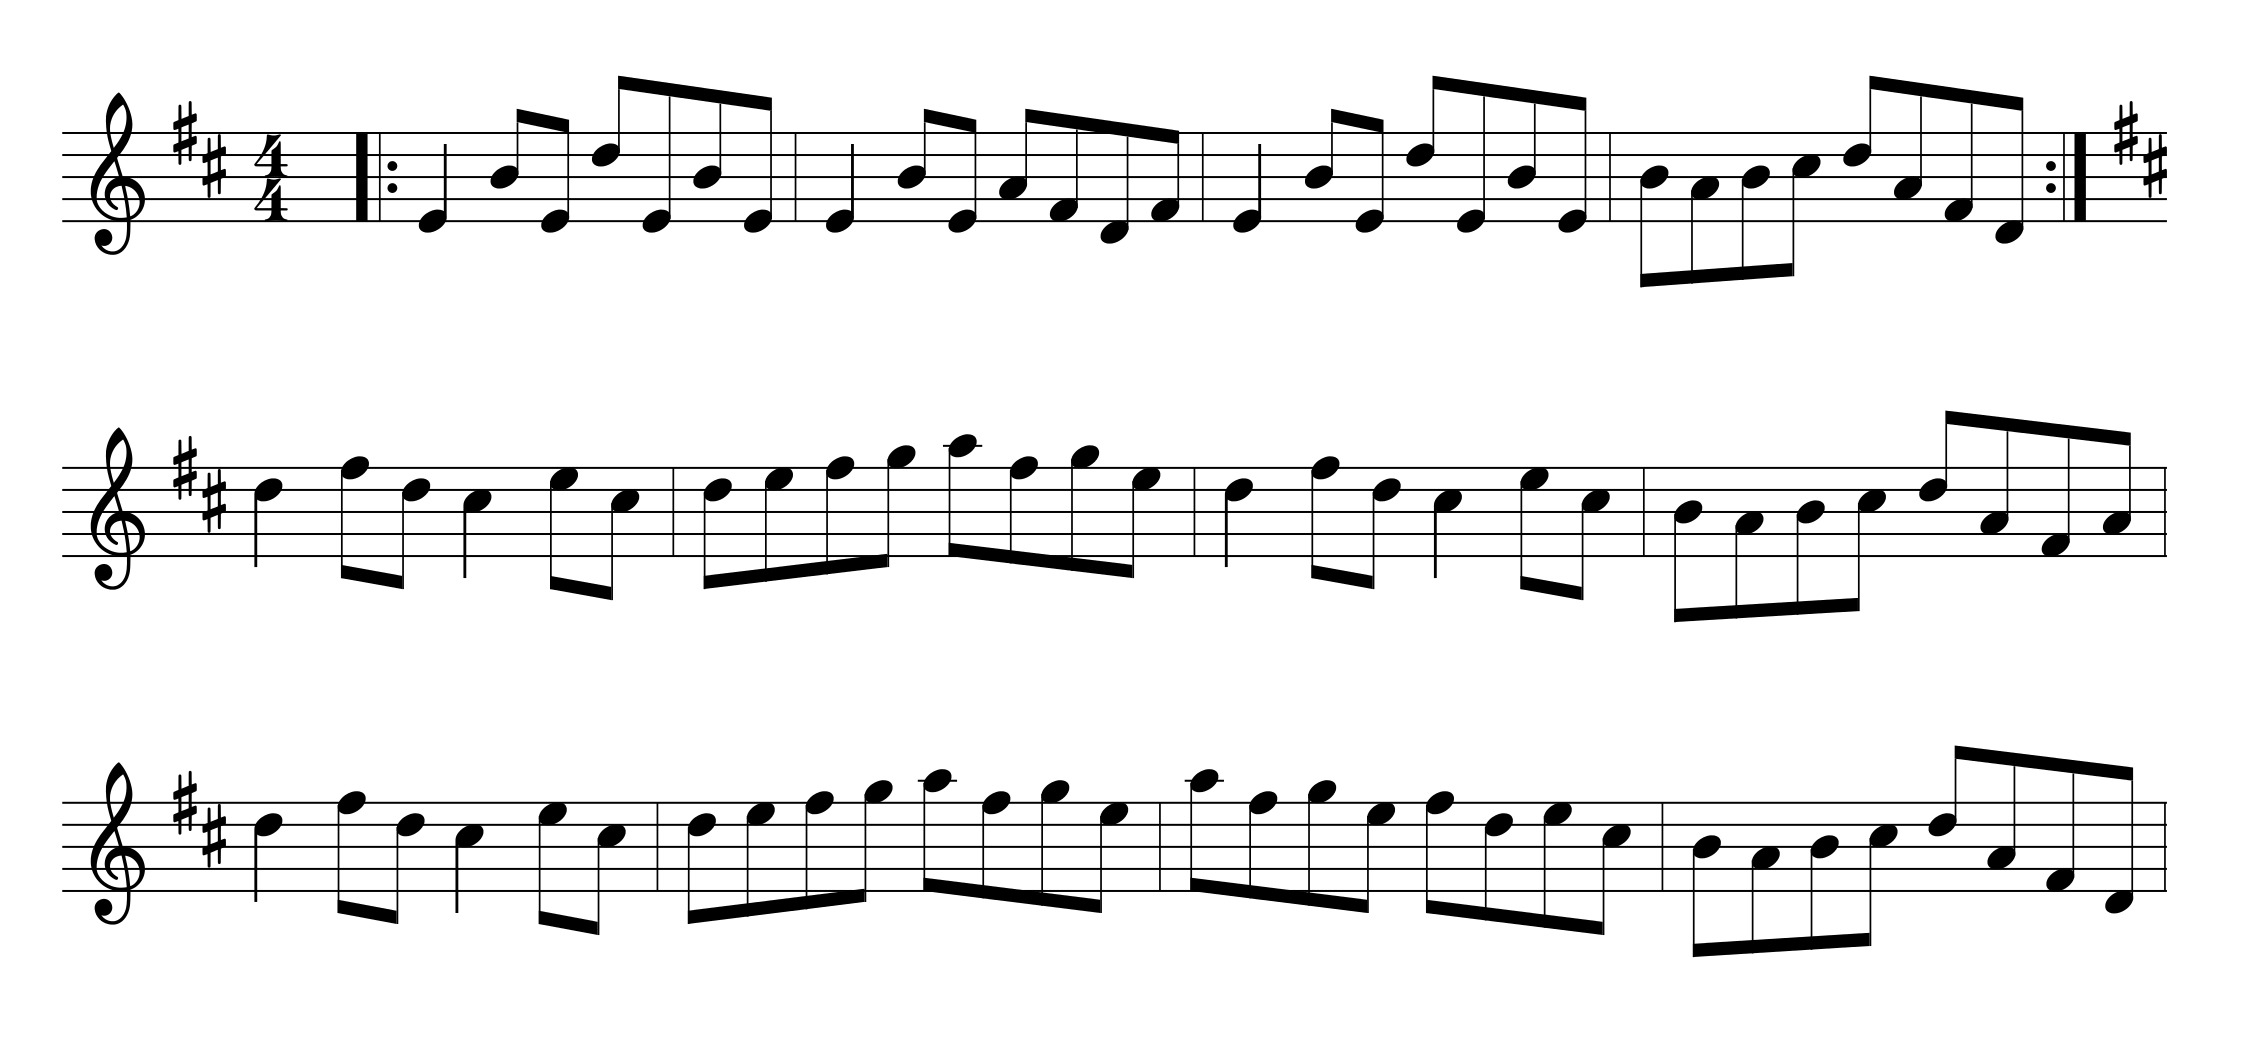
\includegraphics[width=5in]{drowsymaggie.png}
  \end{center}
  \caption{A rendering of \textit{Drowsy Maggie} in standard musical notation, for
  comparison with ABC notation. The $A$ section of this tune can be seen in the
first line, while the $B$ section spans the second and third line. The $A$ and
$B$ sections are the same length since the first four bars are repeated.}
\end{figure}
\FloatBarrier


\end{document}
%TODO: Check names of tunes against each other
%TODO: Check these numbers
